%%%%%%%%%%%%%%%%%%%%%%%%%%%%%%%%%%%%%%%%%
% Jacobs Landscape Poster
% LaTeX Template
% Version 1.1 (14/06/14)
%
% Created by:
% Computational Physics and Biophysics Group, Jacobs University
% https://teamwork.jacobs-university.de:8443/confluence/display/CoPandBiG/LaTeX+Poster
% 
% Further modified by:
% Nathaniel Johnston (nathaniel@njohnston.ca)
%
% This template has been downloaded from:
% http://www.LaTeXTemplates.com
%
% License:
% CC BY-NC-SA 3.0 (http://creativecommons.org/licenses/by-nc-sa/3.0/)
%
%%%%%%%%%%%%%%%%%%%%%%%%%%%%%%%%%%%%%%%%%

%----------------------------------------------------------------------------------------
%	PACKAGES AND OTHER DOCUMENT CONFIGURATIONS
%----------------------------------------------------------------------------------------

\documentclass[final]{beamer}

\usepackage[scale=1.1]{beamerposter} % Use the beamerposter package for laying out the poster
\usetheme{confposter} % Use the confposter theme supplied with this template
\setbeamercolor{block title}{fg=ngreen,bg=white} % Colors of the block titles
\setbeamercolor{block body}{fg=black,bg=white} % Colors of the body of blocks
\setbeamercolor{block alerted title}{fg=white,bg=dblue!70} % Colors of the highlighted block titles
\setbeamercolor{block alerted body}{fg=black,bg=dblue!10} % Colors of the body of highlighted blocks
% Many more colors are available for use in beamerthemeconfposter.sty

%-----------------------------------------------------------
% Define the column widths and overall poster size
% To set effective sepwid, onecolwid and twocolwid values, first choose how many columns you want and how much separation you want between columns
% In this template, the separation width chosen is 0.024 of the paper width and a 4-column layout
% onecolwid should therefore be (1-(# of columns+1)*sepwid)/# of columns e.g. (1-(4+1)*0.024)/4 = 0.22
% Set twocolwid to be (2*onecolwid)+sepwid = 0.464
% Set threecolwid to be (3*onecolwid)+2*sepwid = 0.708

\newlength{\sepwid}
\newlength{\onecolwid}
\newlength{\twocolwid}
\newlength{\threecolwid}
\setlength{\paperwidth}{45in} % A0 width: 46.8in
\setlength{\paperheight}{42in} % A0 height: 33.1in
\setlength{\sepwid}{0.005\paperwidth} % Separation width (white space) between columns
\setlength{\onecolwid}{0.22\paperwidth} % Width of one column
\setlength{\twocolwid}{0.445\paperwidth} % Width of two columns%was 0.464
\setlength{\threecolwid}{0.67\paperwidth} % Width of three columns
\setlength{\topmargin}{-0.5in} % Reduce the top margin size
%-----------------------------------------------------------

\usepackage{graphicx}  % Required for including images

\usepackage{booktabs} % Top and bottom rules for tables

%----------------------------------------------------------------------------------------
%	TITLE SECTION 
%----------------------------------------------------------------------------------------

\title{A Monte-Carlo based approach for estimating \\remote sensing reflectance uncertainty} % Poster title

\author{Erdem M. Karak\"{o}yl\"{u} \and Bryan Franz} % Author(s)
\institute{NASA Goddard Space Flight Center, Greenbelt, MD, 20771} % Institution(s)

%----------------------------------------------------------------------------------------

\begin{document}

\addtobeamertemplate{block end}{}{\vspace*{2ex}} % White space under blocks
\addtobeamertemplate{block alerted end}{}{\vspace*{2ex}} % White space under highlighted (alert) blocks

%\setlength{\belowcaptionskip}{2ex} % White space under figures
\setlength\belowdisplayshortskip{2ex} % White space under equations

\begin{frame}[t] % The whole poster is enclosed in one beamer frame

\begin{columns}[t] % The whole poster consists of three major columns, the second of which is split into two columns twice - the [t] option aligns each column's content to the top

%\begin{column}{\sepwid}\end{column} % Empty spacer column

\begin{column}{\onecolwid} % The first column

%----------------------------------------------------------------------------------------
%	OBJECTIVES
%----------------------------------------------------------------------------------------

\begin{alertblock}{Objectives}

\begin{itemize}
\item Implement self-contained sensor-dependent (SeaWiFS showcased) noise model.
\item Characterize noise propagation due to atmospheric correction.
\item Characterize impact of noise in near-infrared bands
\item Generate remote sensing reflectance uncertainty product.
\end{itemize}

\end{alertblock}

%----------------------------------------------------------------------------------------
%	INTRODUCTION
%----------------------------------------------------------------------------------------

\begin{block}{Introduction}
\begin{itemize}
\item Satellite borne ocean color remote sensors measure \textbf{top of the atmosphere radiance ($L_t$)}
\item $L_t$ is used to derive \textbf{remote sensing reflectance ($Rrs$)}, from which other  properties of interest are obtained.
\item Along the way, uncertainties are accumulated, but remain illusive as they are difficult to estimate consistently.
\item Typical uncertainty estimation done using potentially problematic comparisons with in-situ data or other remote sensing missions\cite{BW:2006,Tle:2000,Hu:2013}.
\item These problems arise because of spatial and temporal scale differences between measurements, and the uncertainties inherent in the reference methods.
\item To begin addressing uncertainties in a consistent manner, a self-contained approach is needed to tease out the some of the noise that contributes to the overall uncertainty budget.
\end{itemize}
\end{block}


%----------------------------------------------------------------------------------------
%	METHODS - ditch that change to Approach
%----------------------------------------------------------------------------------------

\begin{block}{Approach}
\begin{itemize}
\item Signal-to-noise Ratio (SNR) is modeled as a function of measured $L_t$, following \cite{Barnes:1994}.
\item Spread in noise distribution given by $\sigma = \frac{L_t}{SNR}$.
\item $L_{t,NOISE} = \mathcal{N}(L_t, \sigma)$
\item Propagate noise through atmospheric correction, retrieve remote sensing reflectance ($Rrs$).
\item Use steps above to run Monte-Carlo Simulation.
\end{itemize}
\end{block}


\begin{figure}
\centering
\textbf{Matching $L_t$ to shot noise via SNR model}\par\medskip
%
\includegraphics[width=1.0\linewidth]{placeholder.jpg}
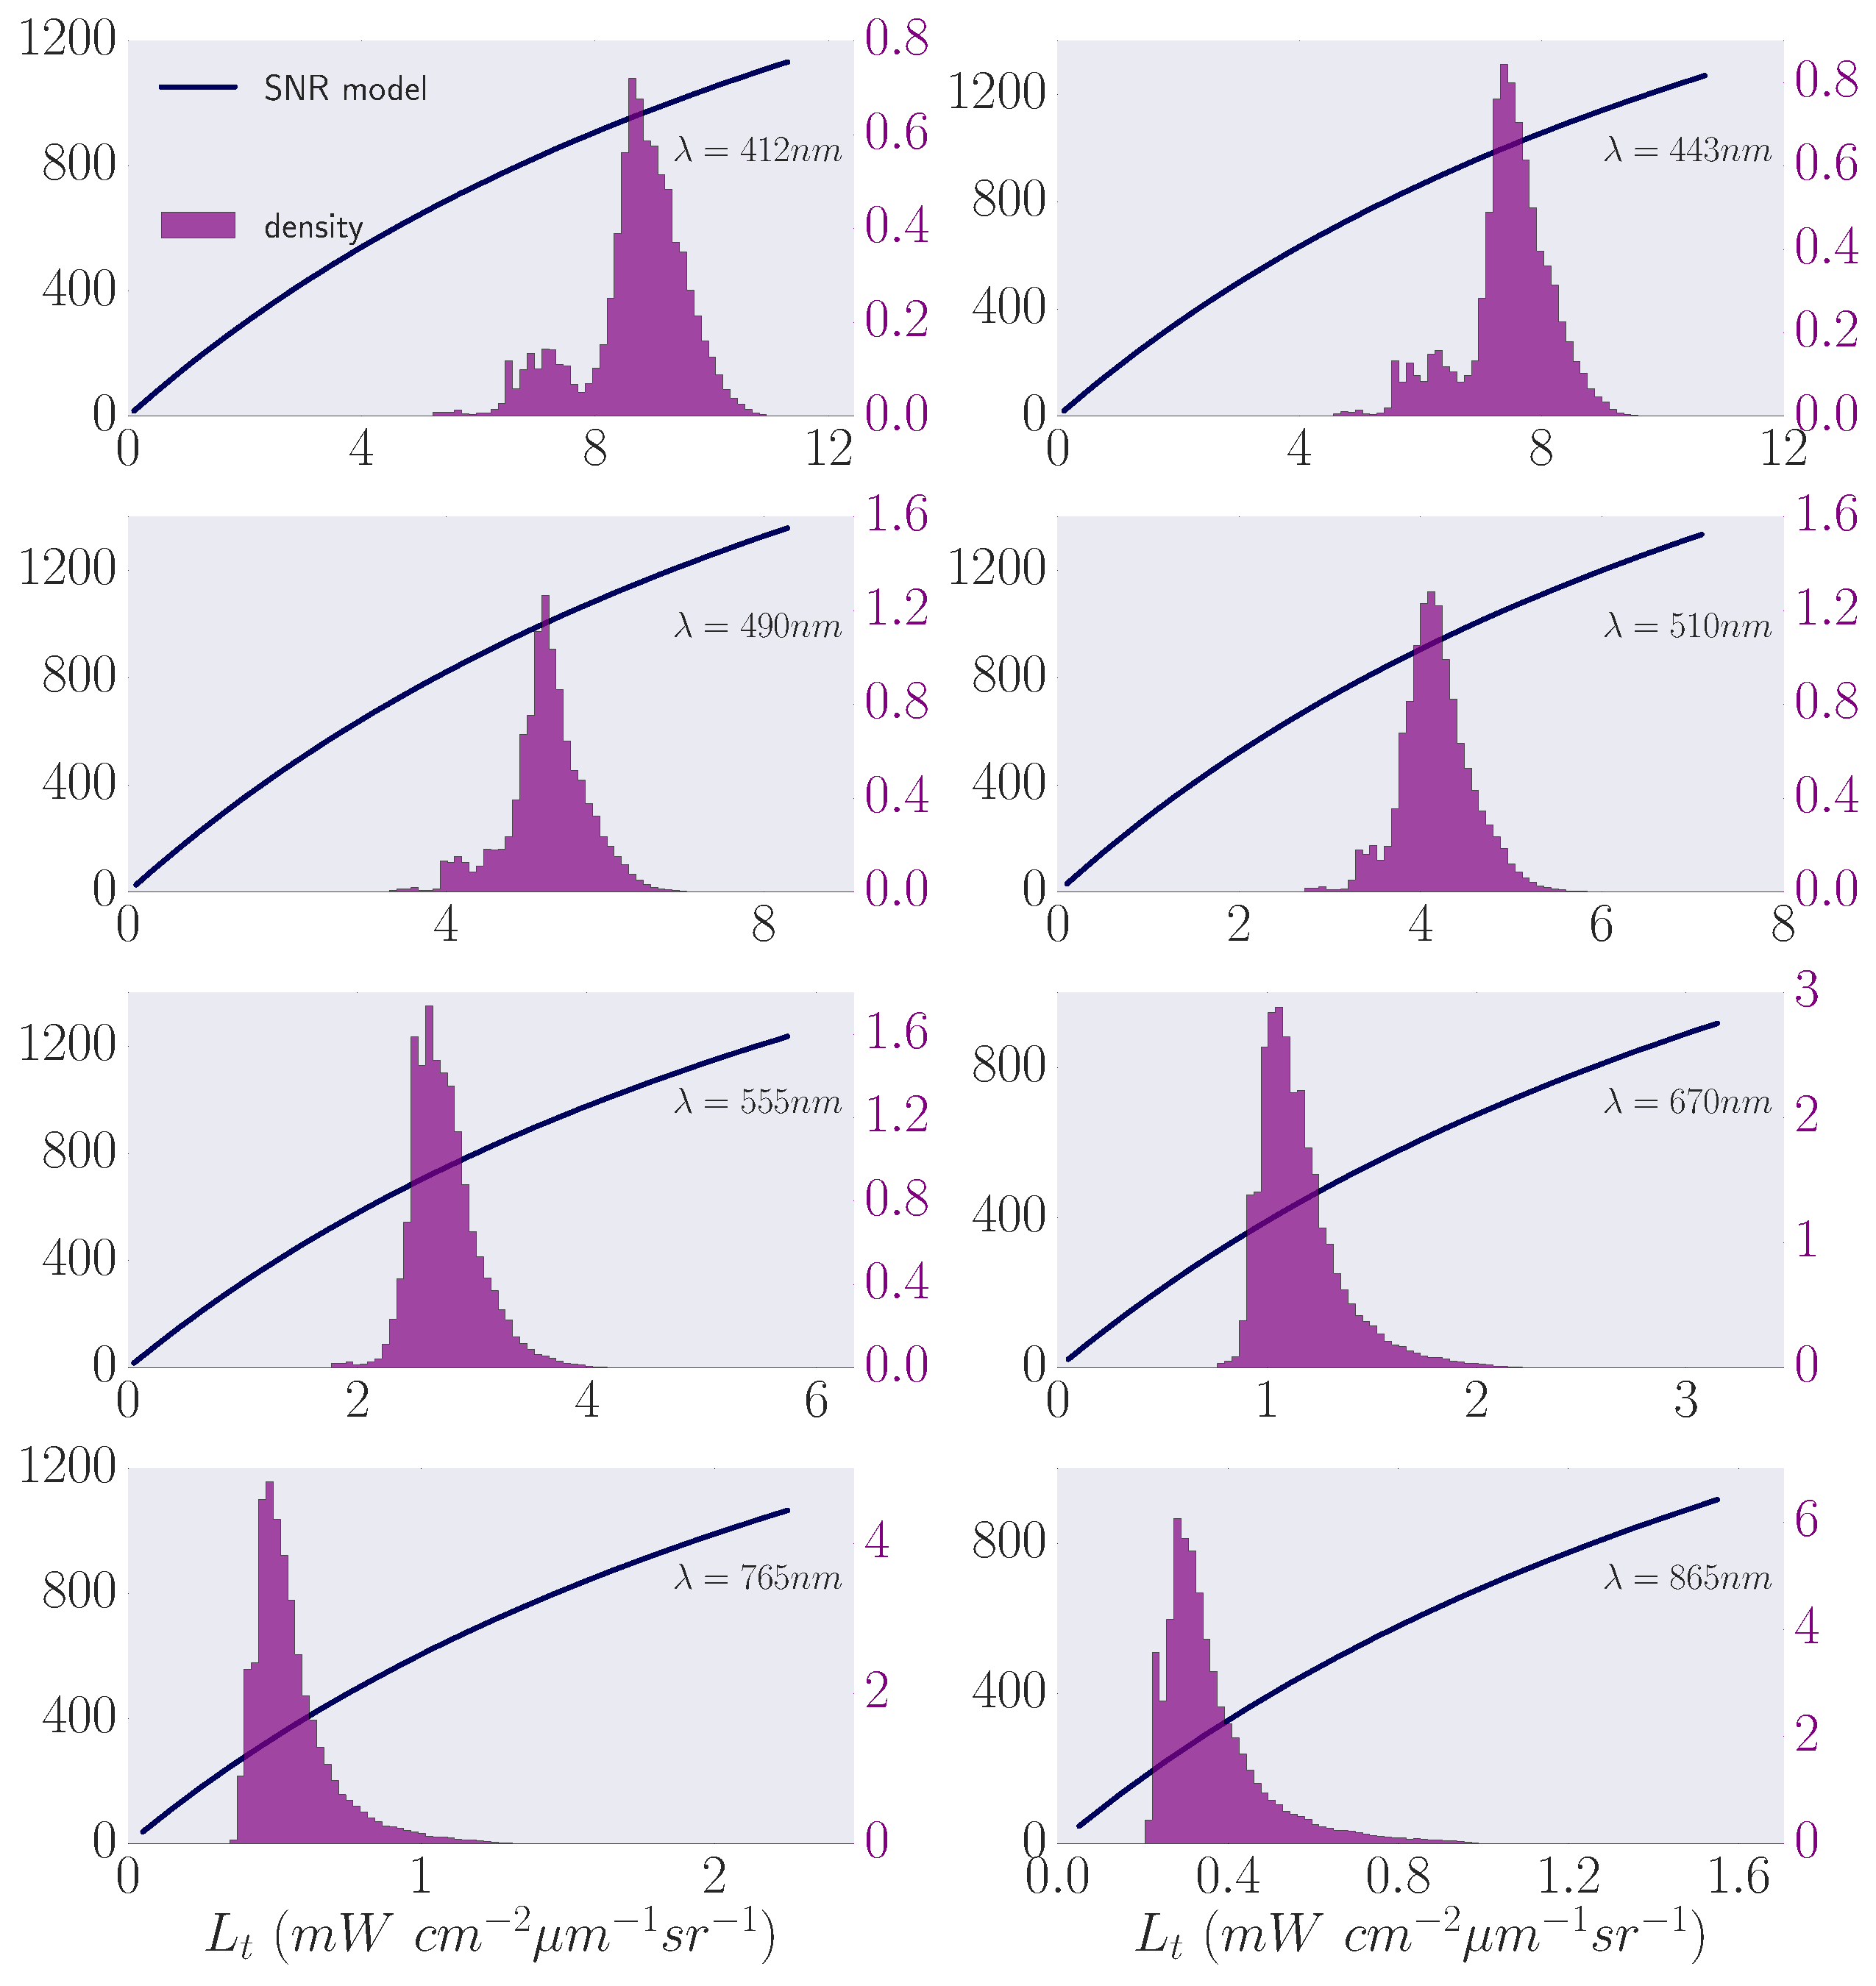
\includegraphics[width=1.0\linewidth]{snrmodelLong.pdf}
\\{For each pixel in a scene (purple histogram) $L_t(\lambda)$  is matched to a  corresponding noise  model parameter $\sigma$ by way of an SNR model. $\sigma$ then drives the}
\end{figure}


\end{column} % End of the first column

%\begin{column}{0.5\sepwid}\end{column} % Empty spacer column

\begin{column}{\twocolwid} % Begin a column which is two columns wide (column 2)
%----------------------------------------------------------------------------------------
%	RESULTS - remove sensitivity analysis figures here, 
%  Do some side by side comparisons of distributions of 
%  Rrs_unc for 
%----------------------------------------------------------------------------------------
\begin{block}{Results}

% Add sensitivity analysis after this, just one of the plots.
\begin{columns}[t,totalwidth=\twocolwid] % Split up the two columns wide column
% text here?
\begin{column}{\onecolwid}\vspace{-.6in} 
%------------------------------ The first column within column 2 (column 2.1)

\begin{table}
\centering
\vspace{2ex}
\caption{Results of sensitivity analysis for a selection of bands}
\begin{tabular}{|*{7}{c|}}
\toprule
\textbf{Perturbed} & \multicolumn{6}{|c|}{\textbf{\% change in Rrs}}\\
\cline{2-7}
\textbf{Lt} (+0.1\%) & \textbf{412} & \textbf{443} & \textbf{490} & \textbf{510} & \textbf{555} & \textbf{670}\\
\midrule
Lt(412) &  1.14 & -- & -- & -- & -- & --\\  
Lt(443) & 0.22 & 0.97 & 0.21 & 0.22 & 0.22 &  0.53\\
Lt(490) & 0.22 & 0.21 & 0.79 & 0.22 & 0.23 &  0.93\\
Lt(510) & 0.97 & 0.62 & 0.41 &  1.0 & 0.35 & 0.84\\
Lt(555) & 0.23 & 0.22 & 0.23 & 0.24 & 1.6 & 1.2\\
Lt(670) & 0.51 & 0.38 & 0.27 & 0.32 & 0.31 &  5.0\\
Lt(765) & 0.90 & 0.92 & 0.95 &  1.5 &  2.4 &  7.5\\
Lt(865) & 0.66 & 0.65 & 0.65 &  1.0 &  1.5 &  4.3\\
\bottomrule
\end{tabular}
\\{blah blah blah Caption caption caption}
\end{table}
%---------- First Global ------------------------
\begin{figure}
\vspace{5in}
\centering
\textbf{Rrs(412) uncertainty}\par\medskip
\includegraphics[width=1.0\linewidth]{rrsPercUnc412.png}
\end{figure}
\end{column} 
% --------------------------- End of column 2.1

\begin{column}{\onecolwid}\vspace{-.6in} % The second column within column 2 (column 2.2)


\begin{figure}
\vspace{2ex}
\caption{My Title}\par%\medskip
\vspace{-1in}
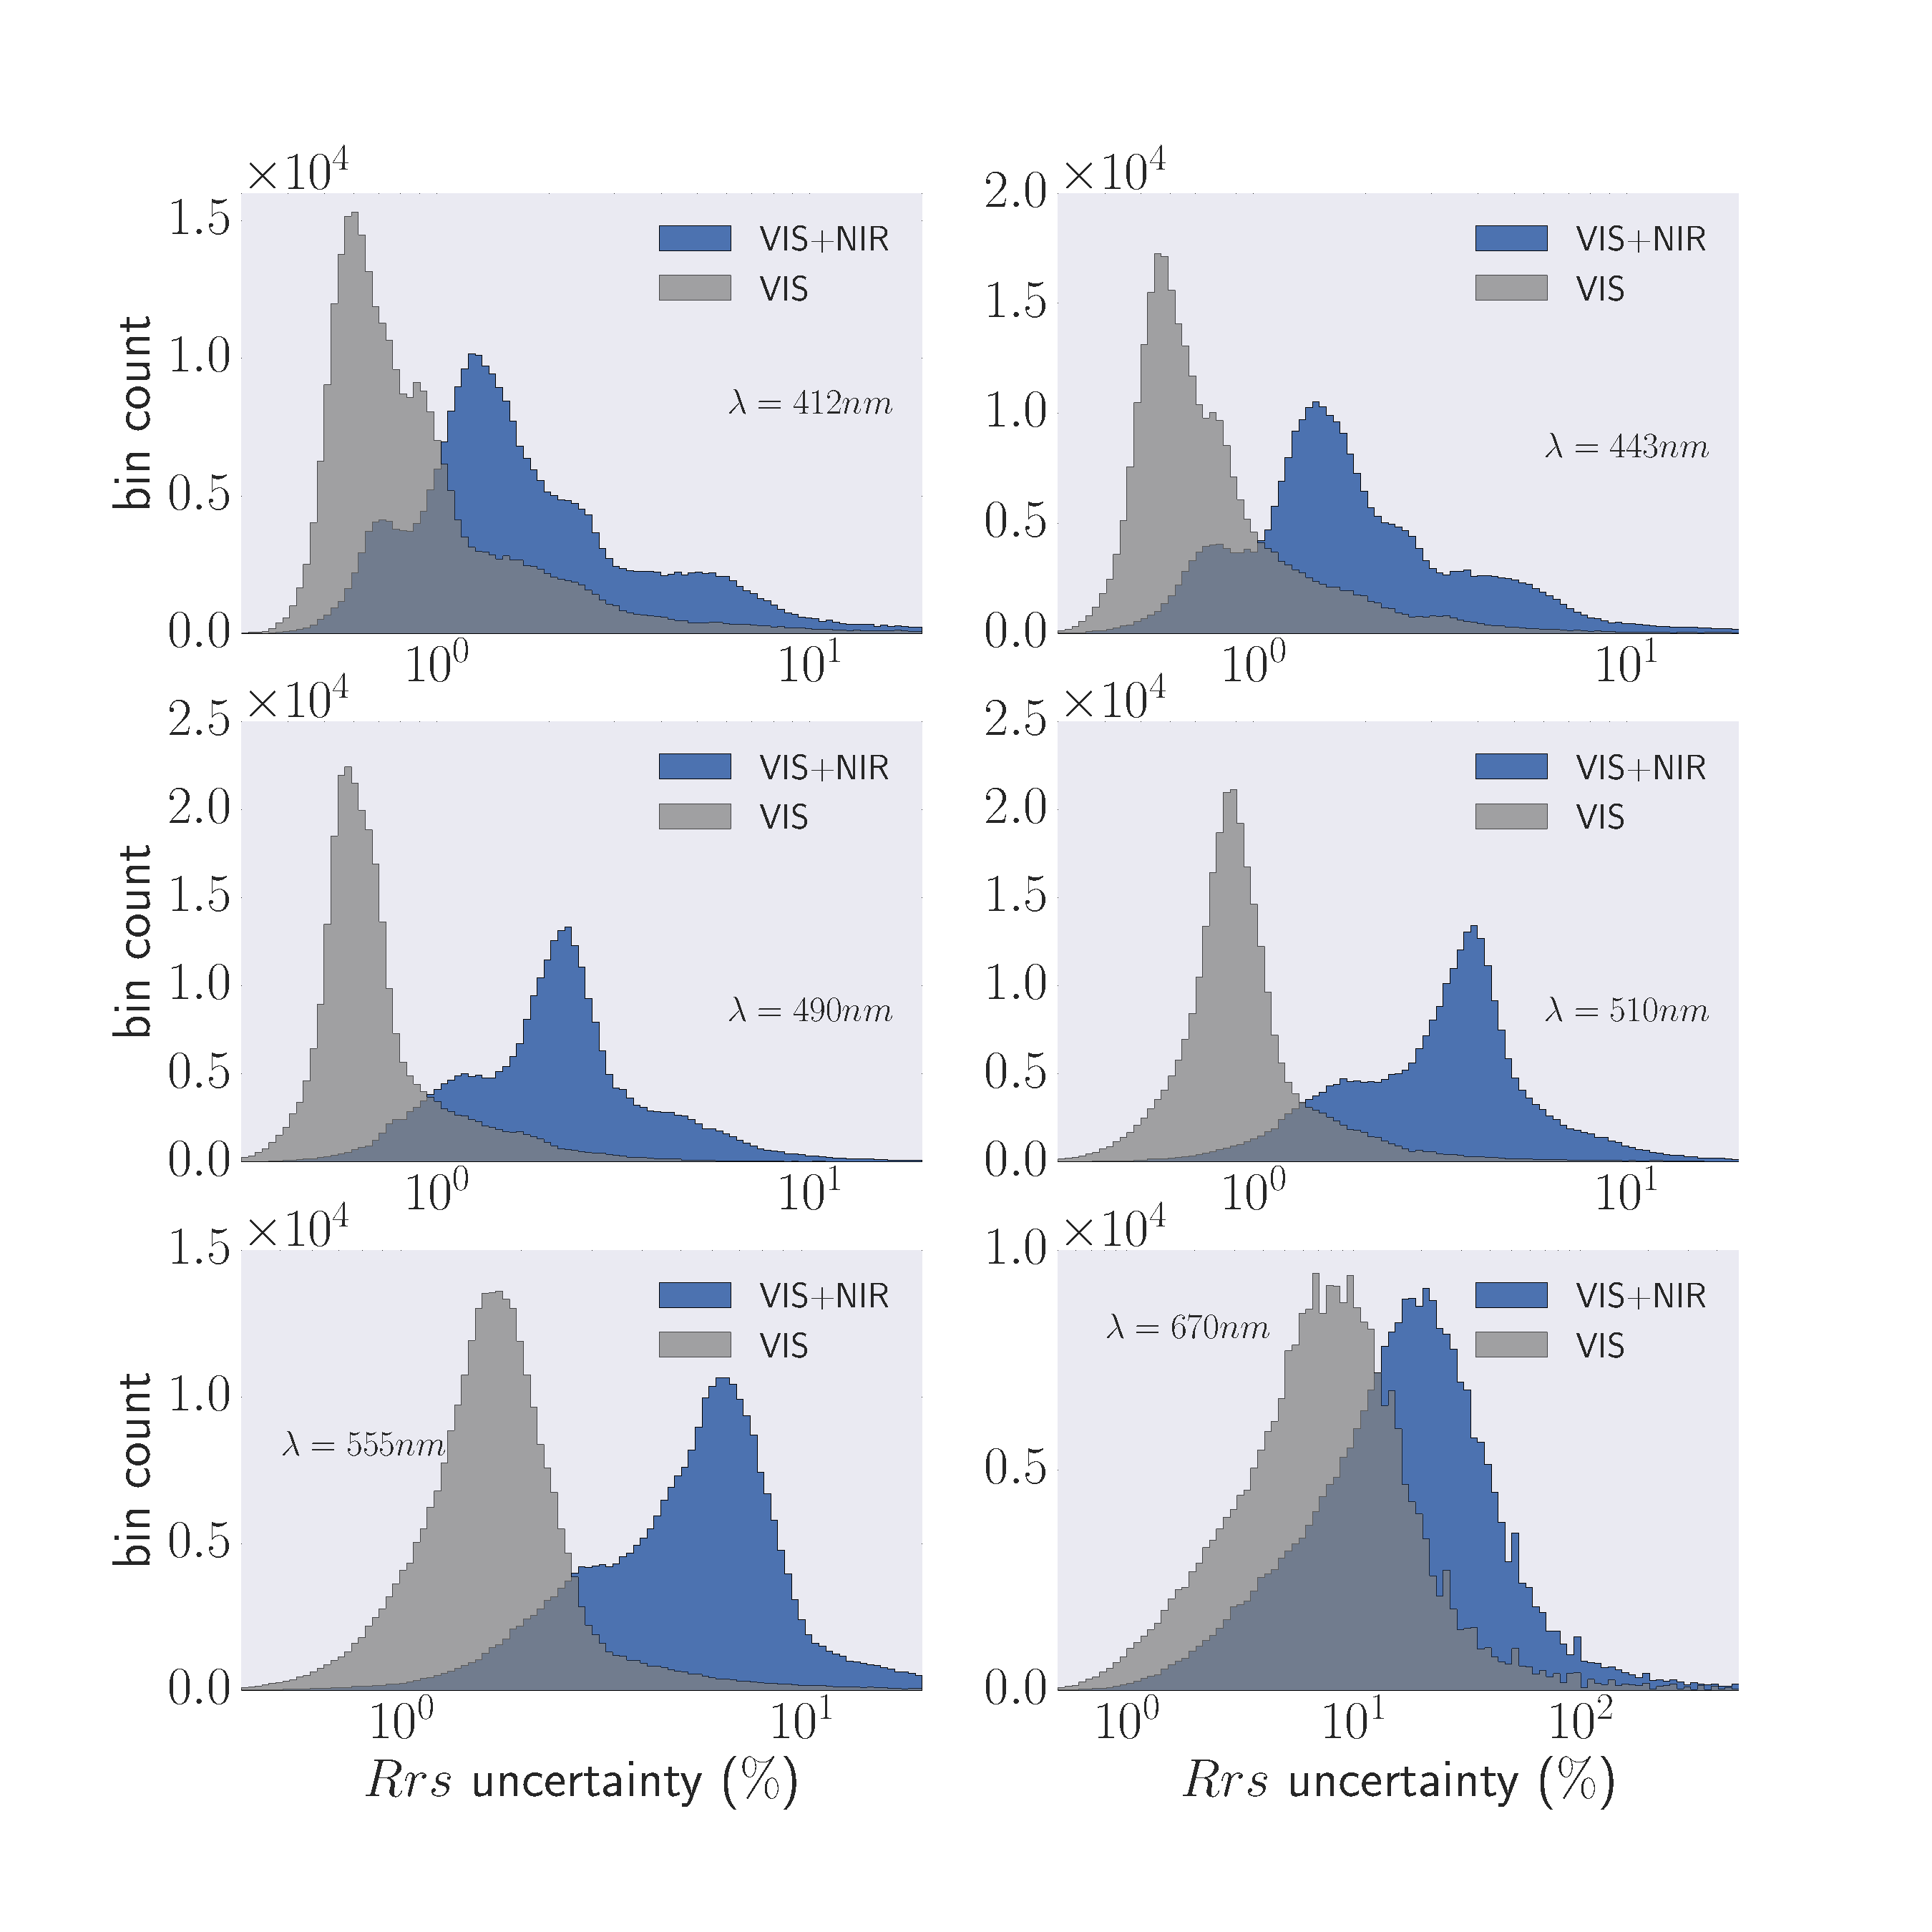
\includegraphics[width=1.0\linewidth]{Vis_vs_VISNIR.pdf}
\end{figure}
%----------- Second Global -------------------
\begin{figure}
\centering
\textbf{Rrs(555) uncertainty}\par\medskip
\includegraphics[width=1.0\linewidth]{rrsPercUnc555.png}
\end{figure}
\end{column} % End of column 2.2

\end{columns} % End of the split of column 2 - any content after this will now take up 2 columns width
\end{block}
% global412 was here
%---------- Colorbar ------------------------
\begin{figure}
\centering

\includegraphics[width=1.0\linewidth]{rrsUNCcolorbar.png}
\\{Rrs uncertainty (\%)}\par\medskip
\end{figure}
%global555 was here


\begin{columns}[t,totalwidth=\twocolwid] % Split up the two columns wide column again
\begin{column}{\onecolwid} % The first column within column 2 (column 2.1)






%----------------------------------------------------------------------------------------

\end{column} % End of column 2.2

\end{columns} % End of the split of column 2

\end{column} % End of the second column

%\begin{column}{\sepwid}\end{column} % Empty spacer column

\begin{column}{\onecolwid} % The third column

%----------------------------------------------------------------------------------------
%	What's next?
%----------------------------------------------------------------------------------------

\begin{block}{Next Steps}
\begin{itemize}
\item Extend MC simulations to other sensors.
\item MC simulations computationally costly;
	\begin{itemize}
	\item Finding an alternative to build on this work, a priority
	\item Develop machine learning (ML) approach (e.g. neural network);
	\item Identify uncertainty drivers in MC as potential inputs to ML;
 	\item Use ML to shorten uncertainty product generation to one run. 
	\end{itemize}
\end{itemize}

\end{block}


%----------------------------------------------------------------------------------------
%	REFERENCES
%----------------------------------------------------------------------------------------

\begin{block}{References}
\nocite{} % Insert publications even if they are not cited in the poster
\small{\bibliographystyle{IEEEtran}
\bibliography{poster}\vspace{0.75in}}

\end{block}

%----------------------------------------------------------------------------------------
%	ACKNOWLEDGEMENTS
%----------------------------------------------------------------------------------------

\setbeamercolor{block title}{fg=red,bg=white} % Change the block title color

\begin{block}{Acknowledgements}

\small{\rmfamily{We thank \textit{Don Shea} and \textit{Sean Bailey} for assistance with l2gen integration of the MC code, and to \textit{Tommy Owens} for running large scale MC simulations on the OBPG production system.}} \\

\end{block}

%----------------------------------------------------------------------------------------
%	CONTACT INFORMATION
%----------------------------------------------------------------------------------------

\setbeamercolor{block alerted title}{fg=black,bg=norange} % Change the alert block title colors
\setbeamercolor{block alerted body}{fg=black,bg=white} % Change the alert block body colors

\begin{alertblock}{Contact Information}

\begin{itemize}
\item Web: \href{oceancolor.gsfc.nasa.gov}{oceancolor.gsfc.nasa.gov}
\item Email: \href{mailto:erdem.m.karakoylu@nasa.gov}{erdem.m.karakoylu@nasa.gov}
\item Phone: +1 (301) 286 0501
\end{itemize}

\end{alertblock}

\begin{center}
\begin{tabular}{ccc}

\includegraphics[width=0.4\linewidth]{NASA_logo.png} & \hfill 
\end{tabular}
\end{center}

%----------------------------------------------------------------------------------------

\end{column} % End of the third column
\begin{column}{\sepwid}\end{column} % Empty spacer column
\end{columns} % End of all the columns in the poster

\end{frame} % End of the enclosing frame

\end{document}
